%% Manuscrito en español con la clase IEEEtran (modo journal), apto para IEEE Revista
%% Iberoamericana de Tecnologías del Aprendizaje (IEEE-RITA) o IEEE Latin America Transactions.
%% Compilar con: latexmk -pdf main_es.tex
\documentclass[journal]{IEEEtran}

\usepackage[T1]{fontenc}
\usepackage[utf8]{inputenc}
\usepackage[spanish,es-tabla,es-noshorthands]{babel}
\usepackage{amsmath,amssymb}
\usepackage{graphicx}
\usepackage{booktabs}
\usepackage{multirow}
\usepackage{array}
\usepackage{textcomp}
\usepackage{url}
\usepackage[hidelinks]{hyperref}
\hypersetup{pdftitle={Efecto de un sistema multiagente de mentoría metodológica en la calidad de proyectos de tesis de ingeniería},pdfauthor={Aguilar Idrogo, Aguilar Alayo, Cueva Chávez}}

% Rótulos al estilo IEEE en español
\addto\captionsspanish{%
  \renewcommand{\tablename}{TABLA}%
  \renewcommand{\figurename}{Fig.}%
  \renewcommand{\refname}{Referencias}%
  \renewcommand{\abstractname}{Resumen}%
}

\newcolumntype{L}[1]{>{\raggedright\arraybackslash}p{#1}}
\newcolumntype{C}[1]{>{\centering\arraybackslash}p{#1}}

\begin{document}

\title{Efecto de un sistema multiagente de mentoría metodológica basado en modelos de lenguaje en la calidad de proyectos de tesis de ingeniería: un cuasiexperimento longitudinal}

\author{Clever~Josu\'e~Aguilar~Idrogo,
        Alessia~Vidamilagros~Aguilar~Alayo
        y~Walter~Manuel~Cueva~Ch\'avez%
\thanks{Manuscrito recibido el 5 de noviembre de 2026. Esta investigación no recibió financiamiento externo. \textit{(Autor de correspondencia: Clever Josu\'e Aguilar Idrogo.)}}%
\thanks{Los autores pertenecen al Programa de Estudio de Ingeniería de Computación y Sistemas, Facultad de Ingeniería, Universidad Privada Antenor Orrego, Trujillo 13008, Perú (correo electrónico: cleverjosue1@gmail.com).}%
\thanks{Título en inglés: \emph{Effect of a Multi-Agent LLM-Based Methodological Mentoring System on the Quality of Engineering Thesis Projects: A Longitudinal Quasi-Experiment}.}}

\markboth{IEEE Revista Iberoamericana de Tecnologías del Aprendizaje}%
{Aguilar Idrogo \MakeLowercase{\textit{et al.}}: Mentoría metodológica multiagente y calidad de proyectos de tesis en ingeniería}

\maketitle

\begin{abstract}
Los proyectos de tesis de pregrado en ingeniería son devueltos con frecuencia con observaciones metodológicas. Este estudio determinó el efecto de MentorIA, un sistema multiagente de mentoría metodológica basado en modelos de lenguaje, en la calidad metodológica de los proyectos de tesis del curso Proyecto de Investigación de una facultad de ingeniería peruana durante el semestre 2026-2. Se aplicó un diseño mixto, cuasiexperimental longitudinal con grupo de control no equivalente, a dos secciones intactas a cargo del mismo docente (16 proyectos de tesis en el grupo de control y 20 en el experimental). La mentoría tradicional se diagnosticó mediante entrevistas a seis asesores. La calidad se midió de la semana 4 a la semana 9 con una rúbrica dicotómica de 100 ítems en 15 dimensiones, validada por siete expertos (V de Aiken entre .81 y 1.00) y aplicada por un panel ciego de tres jueces basados en modelos de lenguaje con voto de mayoría; la calidad argumentativa se evaluó con el modelo de Toulmin. En la medición inicial los grupos no difirieron en la calidad del núcleo común de dimensiones (71.2\,\% frente a 78.5\,\%, $p = .057$), pero sí en la trazabilidad, a favor del grupo de control. La calidad aumentó en 32 de 36 proyectos (mediana $+13.0$ puntos, $p < .001$). La pendiente semanal del grupo experimental fue 3.10 puntos mayor ($p < .001$) y el efecto sobre el cambio de la calidad fue grande ($d$ de Cohen $= 1.32$, IC 95\,\% $[0.60, 2.05]$), concentrado en la descripción del problema y en las dimensiones redactadas durante la intervención. El uso acumulado (215 consultas) no se relacionó con la mejora ($\rho = -.14$). Disponer del sistema como complemento de la asesoría se asoció con una evolución más favorable de la calidad metodológica, sin evidencia de una relación de dosis y respuesta.
\end{abstract}

{\renewcommand{\IEEEkeywordsname}{Palabras clave}%
\begin{IEEEkeywords}
Asesoría de tesis, calidad metodológica, cuasiexperimento, educación superior, minería de argumentos, modelos de lenguaje, sistemas multiagente.
\end{IEEEkeywords}}

{\renewcommand{\abstractname}{Abstract}%
\begin{abstract}
Undergraduate engineering thesis projects are frequently returned with methodological observations. This study determined the effect of MentorIA, a multi-agent methodological mentoring system based on large language models, on the methodological quality of thesis projects in a Research Project course at a Peruvian engineering faculty during the 2026-2 semester. A mixed-methods, longitudinal quasi-experimental design with a nonequivalent control group was applied to two intact sections taught by the same instructor (16 control and 20 experimental thesis projects). Traditional mentoring was diagnosed through interviews with six advisors. Quality was measured in weeks 4 to 9 with a 100-item dichotomous rubric in 15 dimensions, validated by seven experts (Aiken's $V$ between .81 and 1.00) and applied by a blind panel of three language-model judges with majority voting; argumentative quality was assessed with Toulmin's model. At baseline the groups did not differ in the quality of the common core of dimensions (71.2\% vs. 78.5\%, $p = .057$) but did in traceability, favoring the control group. Quality increased in 32 of 36 projects (median $+13.0$ points, $p < .001$). The weekly slope of the experimental group was 3.10 points higher ($p < .001$), and the effect on the change in quality was large (Cohen's $d = 1.32$, 95\% CI $[0.60, 2.05]$), concentrated in the problem description and in the dimensions written during the intervention. Cumulative use (215 queries) was unrelated to improvement ($\rho = -.14$). Availability of the system as a complement to advising was associated with a more favorable evolution of methodological quality, without evidence of a dose--response relationship.
\end{abstract}}

\begin{IEEEkeywords}
Argument mining, higher education, large language models, methodological quality, multi-agent systems, quasi-experiment, thesis supervision.
\end{IEEEkeywords}

\IEEEpeerreviewmaketitle

\section{Introducción}

\IEEEPARstart{E}{n} la Facultad de Ingeniería de la Universidad Privada Antenor Orrego (UPAO), el curso Proyecto de Investigación es la etapa en la que los estudiantes del Programa de Ingeniería de Computación y Sistemas formulan el proyecto de tesis con el que optarán al título profesional, bajo un modelo de asesoría individualizada. Ese modelo presenta una limitación estructural: la asesoría se organiza en sesiones programadas dentro de un horario fijo y no ofrece un canal de orientación metodológica en el momento en que surge la duda, de modo que los vacíos no resueltos se acumulan y se propagan a lo largo del documento. A ello se suma una condición propia de la formación en ingeniería: los estudiantes tienden a concebir el proyecto desde la solución tecnológica que desean construir y no desde el problema científico que pretenden resolver, lo que invierte el orden metodológico y produce errores recurrentes en la formulación del problema, la definición de variables y el diseño. Según los asesores de la facultad, más de la mitad de los proyectos presentados en primera instancia son devueltos con observaciones de fondo metodológico. El problema no es exclusivo de una institución: en una universidad pública peruana, el 80\,\% de las tesis de pregrado aprobadas presentó una calidad metodológica apenas regular, con deficiencias atribuidas en parte a la orientación recibida \cite{estrada2022}, y los estudios sobre las dificultades del tesista peruano se han construido desde el documento terminado o desde la voz del estudiante, sin la perspectiva de quien asesora \cite{perdomo2022,vilca2023}. La supervisión de tesis de pregrado, además, ha recibido mucha menos atención investigativa que la doctoral \cite{agricola2021}.

Los agentes conversacionales pedagógicos se han propuesto como mecanismo de acompañamiento continuo, personalizado y escalable en la educación superior, con aplicaciones que incluyen la mentoría \cite{yusuf2025}. La evidencia sobre su efecto en la escritura de investigación, sin embargo, es heterogénea y depende de la arquitectura de la herramienta. Un agente conversacional sin arquitectura especializada tendió a operar como un dispensador de recursos y no sostuvo interacciones de profundidad cognitiva en la tutoría de proyectos de investigación \cite{ortega2021}; un chatbot básico tuvo una adopción limitada y fallos frecuentes ante consultas de contenido complejo en un curso de investigación académica en Lima \cite{arredondo2020}; y el uso espontáneo de ChatGPT no produjo diferencias significativas en la calidad de textos académicos frente a un grupo de control no equivalente \cite{apolin2024}. En cambio, una intervención estructurada en cuatro sesiones con ChatGPT elevó del 2.8\,\% al 80.6\,\% la proporción de estudiantes de posgrado con un nivel adecuado en la formulación de proyectos de investigación, aunque con un diseño preexperimental sin grupo de comparación \cite{hinojosa2024}. Una revisión sistemática con metaanálisis recomienda evaluar estos efectos a lo largo del tiempo para distinguirlos de un efecto de novedad \cite{deng2025}.

Los sistemas multiagente basados en modelos de lenguaje (LLM, por sus siglas en inglés) ofrecen una alternativa a la asistencia conversacional de un único modelo. El debate entre varios agentes que proponen y critican respuestas mejoró la exactitud factual y el razonamiento de los modelos de lenguaje \cite{duy2024}; en un cuasiexperimento con estudiantes de computación, la condición con debate multiagente obtuvo una mejora relativa del aprendizaje del 29.78\,\%, con un tamaño de efecto medio \cite{duj2025}; la separación de roles entre agentes críticos y un juez redujo la sicofancia pedagógica de los tutores automatizados \cite{sadhu2025}; y la descomposición de la evaluación de ensayos en agentes especializados guiados por una rúbrica elevó el acuerdo con calificadores humanos \cite{jordan2025}. Los paneles de jueces basados en modelos de lenguaje, no obstante, presentan un sesgo de autopreferencia cuando el evaluador y el generador pertenecen a la misma familia de modelos \cite{panickssery2024}. Por otro lado, la estructura argumentativa de los textos de estudiantes puede identificarse de forma automática y reproducible \cite{stab2017}, y la retroalimentación sobre esa estructura mejoró la calidad de los textos persuasivos \cite{wambsganss2020}; esos procedimientos, sin embargo, se han desarrollado sobre ensayos y no sobre las secciones argumentativas de un proyecto de investigación.

De la revisión se desprenden cinco brechas. Primera, la escasez de diagnósticos de las deficiencias metodológicas desde la perspectiva del asesor de ingeniería y organizados por sección del proyecto. Segunda, la medición de la calidad metodológica en un único momento o con solo dos mediciones, que no permite describir cuándo se separan las trayectorias de los grupos. Tercera, el predominio de intervenciones con un modelo conversacional único y de propósito general, con escasa evidencia controlada sobre sistemas multiagente especializados. Cuarta, el registro del uso real de las herramientas con fines descriptivos, sin vincularlo con la calidad de un producto de investigación. Quinta, la ausencia de una evaluación computacional de la argumentación en proyectos de investigación y de su relación con la calidad metodológica del documento.

El objetivo general del estudio fue determinar el efecto del uso de un sistema multiagente de mentoría metodológica en la calidad metodológica de los proyectos de tesis de los estudiantes de Ingeniería de la UPAO en el semestre 2026-2. Los objetivos específicos fueron: (OE1) explorar las deficiencias metodológicas recurrentes del proceso de mentoría tradicional desde la perspectiva de los asesores; (OE2) medir la evolución de la calidad metodológica de los proyectos a lo largo de mediciones semanales; (OE3) determinar la relación entre el nivel de uso del sistema y la mejora de la calidad en el grupo experimental; (OE4) comparar la evolución de la calidad entre el grupo de control y el grupo experimental; y (OE5) comparar entre grupos la evolución de la calidad argumentativa de la descripción del problema y de la justificación, evaluada computacionalmente según el modelo de Toulmin. La hipótesis general planteó que el sistema multiagente tiene un efecto positivo y estadísticamente significativo en la calidad metodológica de los proyectos; las hipótesis específicas H2 a H5 plantearon, respectivamente, que la calidad aumenta a lo largo de las mediciones, que el nivel de uso se relaciona positivamente con la mejora, que el grupo experimental presenta una evolución mayor que el de control y que la calidad argumentativa aumenta más en el grupo experimental. Las contribuciones son una evaluación controlada y longitudinal de un sistema multiagente especializado en un curso real, una rúbrica validada por expertos administrada por un panel de LLM con consistencia reportada en cada medición y un índice computacional de argumentación para las secciones de un proyecto de investigación.

\section{Materiales y métodos}

\subsection{Diseño}

Se realizó un estudio de enfoque mixto, de tipo aplicado y alcance explicativo, con un diseño cuasiexperimental longitudinal con grupo de control no equivalente \cite{hernandez2018}. Los grupos fueron dos secciones intactas del curso; cada sección se asignó al azar, en bloque, a una de las dos condiciones. La variable independiente, la exposición al sistema multiagente, se manipuló al ponerlo a disposición únicamente del grupo experimental; la variable dependiente, la calidad metodológica del proyecto de tesis, se midió semanalmente en ambos grupos con el mismo instrumento y el mismo sistema evaluador. El esquema del diseño fue GC: $O_1 \rightarrow O_2 \rightarrow \cdots \rightarrow O_n$; GE: $O_1 \rightarrow X \rightarrow O_2 \rightarrow X \rightarrow \cdots \rightarrow O_n$, donde $O_1$ es la medición inicial de la semana 4, $X$ es el uso del sistema entre mediciones consecutivas y $O_2$ a $O_n$ son las mediciones sucesivas. Como ambos grupos inician el curso con una plantilla institucional sin texto evaluable, la equivalencia se verificó en la medición inicial, cuando ya habían redactado las primeras dimensiones del proyecto. La validez interna se abordó con tres estrategias: la verificación de la homogeneidad inicial sobre el núcleo común de dimensiones desarrolladas por ambos grupos; la comparación de las trayectorias de ambos grupos sobre las mismas dimensiones; y el análisis de dosis y respuesta dentro del grupo experimental, que mantiene constantes los factores propios de la sección.

\subsection{Población y muestra}

La unidad de análisis fue el proyecto de tesis, no el estudiante, dado que la variable dependiente se mide sobre el documento y cada proyecto puede ser elaborado por uno o dos estudiantes. La población estuvo constituida por los proyectos del curso Proyecto de Investigación de la Facultad de Ingeniería de la UPAO en el semestre 2026-2, dictado en tres secciones con 31, 30 y 33 estudiantes matriculados. La muestra, no probabilística e intencional, comprendió las dos secciones a cargo del mismo docente, con el mismo sílabo y calendario de entregas, lo que evita confundir el efecto del docente con el de la intervención; cada sección conformó 20 proyectos y dentro de cada una se incluyeron todos los proyectos cuyos estudiantes autorizaron su participación. Se incluyeron en el análisis los proyectos que presentaron una versión evaluable, con texto propio en al menos una dimensión de la rúbrica, en la medición inicial. Cuatro proyectos del grupo de control conservaban únicamente el formato del curso en esa medición y quedaron fuera de la muestra analítica, que quedó conformada por 36 proyectos: 16 del grupo de control y 20 del grupo experimental. Para el quinto objetivo específico, la unidad de análisis fue la sección argumentativa completa de cada proyecto (descripción del problema y justificación), definida como la que contiene al menos 80 palabras propias con al menos el 60\,\% de ellas en oraciones completas.

\subsection{Intervención: el sistema multiagente MentorIA}

El grupo experimental dispuso, además de la asesoría tradicional, de MentorIA, un sistema multiagente de mentoría metodológica desplegado como aplicación web en la nube, al que cada estudiante accedió con una cuenta individual. El sistema recibe el proyecto del estudiante en formato PDF, Word o texto, lo indexa en un almacén vectorial de sesión y lo evalúa contra una rúbrica estructurada por criterios metodológicos explícitos; el estudiante declara qué partes desea revisar, de modo que lo no entregado no se califica. Su núcleo es una red de agentes basados en LLM con roles separados, orquestada por un supervisor que decide en cada turno qué agente interviene: un Auditor que califica los criterios de la rúbrica con salida estructurada, un Metodólogo que revisa el rigor y la coherencia cruzada entre secciones (problema, objetivos, hipótesis, variables y diseño), un Redactor que propone texto mejorado apoyado en la recuperación aumentada de bibliografía metodológica y una ronda de debate entre el Redactor y los evaluadores, con protección contra bucles. El documento original del estudiante nunca se modifica: las mejoras se presentan como propuestas que el estudiante decide incorporar o no. Hubo cuatro tipos de interacción: consultas rápidas, mejoras rápidas de un fragmento, revisiones de una sección y revisiones completas del proyecto. Conforme a la escala de madurez tecnológica adaptada por el Consejo Nacional de Ciencia, Tecnología e Innovación Tecnológica (CONCYTEC) \cite{concytec2022}, el sistema se ubica en el nivel TRL~7, al estar desplegado y en uso real durante el curso. Su arquitectura, configuración y base de conocimiento permanecieron fijas durante el estudio. El sistema estuvo disponible en modalidad de prueba desde la semana 2; la intervención se computa a partir de la medición inicial, de la semana 5 a la semana 9.

\subsection{Instrumentos y medidas}

\subsubsection{Rúbrica de calidad metodológica}
La calidad metodológica se midió con una rúbrica de 100 ítems dicotómicos (cumple $=$ 1; no cumple $=$ 0) agrupados en 15 dimensiones, construida para el estudio a partir de los criterios de Hernández Sampieri y Mendoza Torres \cite{hernandez2018} y de la definición de calidad metodológica como grado de cumplimiento de los estándares de rigor que sustentan la validez \cite{chacon2023}. Las dimensiones son: título (D1); descripción y delimitación del problema (D2); formulación del problema (D3); objetivos (D4); justificación, importancia y viabilidad (D5); limitaciones (D6); marco teórico (D7); hipótesis (D8); variables y operacionalización (D9); matriz de consistencia (D10); tipo, enfoque y alcance (D11); diseño (D12); población, muestra y muestreo (D13); técnicas e instrumentos de recolección (D14); y técnicas de procesamiento y análisis (D15). Un ítem se califica como cumplido solo cuando el elemento está declarado explícitamente en el texto. La validez de contenido se estableció por juicio de siete expertos con grado de magíster o doctor y entre 4 y 15 años de experiencia en investigación o asesoría de tesis, en dos rondas, siguiendo la planilla de Escobar-Pérez y Cuervo-Martínez \cite{escobar2008}, con el coeficiente V de Aiken \cite{aiken1980} y un criterio de aceptación de $V \geq .80$ por ítem para pertinencia, relevancia y claridad, y por dimensión para suficiencia. En la primera ronda los coeficientes oscilaron entre .67 y 1.00 (media .96) y doce ítems no alcanzaron el criterio; se reformularon 27 ítems sin alterar el número de ítems ni de dimensiones. En la segunda ronda todos los ítems alcanzaron el criterio, con valores entre .81 y 1.00 (media .98) y 55 ítems con $V = 1.00$ en los tres criterios; la suficiencia por dimensión osciló entre .81 y 1.00. La variable principal fue la \emph{calidad de lo redactado}: el porcentaje de criterios cumplidos sobre los criterios de las dimensiones que el proyecto ha desarrollado, lo que separa la calidad de lo escrito de la extensión del avance; cuando el proyecto desarrolla las 15 dimensiones coincide con el puntaje total de 0 a 100. Se derivaron además la calidad en el núcleo común de dimensiones desarrolladas por ambos grupos y la trazabilidad entre título, problema y objetivos, calculada como el porcentaje cumplido de seis ítems de correspondencia.

\subsubsection{Sistema evaluador multiagente}
La rúbrica fue administrada en todas las mediciones por un sistema evaluador construido para el estudio, lo que hizo viable la evaluación semanal de los 40 proyectos y evitó el conflicto de interés de que el asesor calificara a sus propios asesorados. El sistema está compuesto por un panel de tres jueces basados en modelos de lenguaje de distinta capacidad (gpt-4o-mini, gpt-4.1-mini y gpt-4.1), orquestados en una arquitectura de red mediante LangGraph. Cada juez evalúa de manera independiente los ítems de las dimensiones con texto propio del estudiante, restringiendo su juicio a los criterios explícitos del instrumento y a la evidencia textual del documento; el puntaje de cada ítem se obtiene por voto de mayoría. Los tres jueces operan con temperatura 0 y semilla fija. La evaluación es ciega: antes de enviar el texto, el sistema enmascara nombres, documentos de identidad, correos, identificadores ORCID y teléfonos, y ningún juez recibe el nombre del archivo ni el grupo del proyecto. Los ítems de las dimensiones sin texto propio, incluidas las que conservan solo el texto de la plantilla institucional, se registran como no cumplidos sin consultar al panel. Cuando una entrega presenta el mismo texto que la anterior, el proyecto conserva su calificación. Como evidencia de consistencia se reportan, en cada medición, el porcentaje de decisiones unánimes, el kappa de Fleiss \cite{fleiss1971} y el coeficiente AC1 de Gwet \cite{gwet2008}. Conforme a la escala del CONCYTEC \cite{concytec2022}, el sistema evaluador se ubica en el nivel TRL~6, como prototipo funcional operado por los investigadores.

\subsubsection{Índice argumentativo y coherencia global}
El sistema evaluador calcula dos indicadores de coherencia en los que el modelo de lenguaje no asigna la nota: identifica elementos del texto, el sistema los verifica automáticamente y la nota se obtiene con una regla fija. El índice argumentativo se basa en los seis componentes del modelo de Toulmin \cite{toulmin2003}: afirmación, dato, garantía, respaldo, calificador y refutación, cuya presencia distingue un argumento elaborado de una enumeración de afirmaciones y datos \cite{erduran2004,qin2010}. En su versión 2.0, empleada para el quinto objetivo, la sección completa se divide en párrafos y unidades numeradas y el modelo gpt-4.1 (temperatura 0, semilla fija) identifica las afirmaciones del autor y, para cada una, las unidades de cualquier párrafo que actúan como su dato, garantía, respaldo o refutación; el sistema verifica que los identificadores existan y que cada garantía conecte un dato válido de la misma afirmación. Se calculan el \emph{índice estructural} (tipos de componente presentes sobre seis, en porcentaje), el \emph{índice de elaboración} (media, sobre las afirmaciones, de la proporción de los cinco componentes de apoyo que tiene cada una), el nivel argumentativo de 0 a 5 adaptado de Erduran \emph{et al.} \cite{erduran2004} y el perfil de componentes. Su estabilidad test-retest, verificada en 58 secciones de la semana 4, fue del 80.6\,\% en las funciones asignadas a 1\,215 unidades y del 65.4\,\% en los vínculos, con un coeficiente de correlación intraclase CCI(2,1) de .77 en ambos índices, interpretado según Koo y Li \cite{koo2016}. La coherencia global del proyecto se obtiene de las contradicciones entre dos partes del documento que el modelo lista con cita literal y que el sistema conserva solo si ambas citas existen en el texto; la nota de 1 a 5 se asigna por regla según el número y la gravedad de las contradicciones.

\subsubsection{Registro de uso del sistema}
La aplicación efectiva de la intervención se verificó con los registros automáticos del sistema, organizados por proyecto y semana académica: número de consultas por tipo (indicador principal de dosis), días con consultas, minutos en sesiones con consultas y sesiones sin mensajes. Una sesión es un bloque de actividad sin pausas mayores de 30 minutos; los minutos de las sesiones sin mensajes se reportan solo como exposición y se incorporan en un análisis de sensibilidad. Una semana sin consultas se registra con dosis cero. Las cuentas se asignaron a los proyectos a partir de los autores de la carátula y se verificaron con los documentos subidos.

\subsubsection{Entrevista semiestructurada}
Para el primer objetivo se aplicó una guía de entrevista, revisada por juicio de expertos, a seis asesores y revisores de proyectos de tesis de la Facultad de Ingeniería, orientada a identificar deficiencias metodológicas, limitaciones de la mentoría tradicional y funcionalidades esperadas de una herramienta de apoyo. Las transcripciones se procesaron mediante identificación de unidades de significado, codificación, agrupación en categorías y triangulación \cite{vives2021}; el criterio de rigor fue la saturación de categorías y la convergencia entre informantes.

\subsection{Procedimiento}

El curso inició en la semana 1 con la plantilla institucional del proyecto sin contenido. Cada grupo presentó su avance en su sesión semanal de clase, los lunes el grupo experimental y los jueves el grupo de control, de modo que ambos fueron medidos con el mismo número de sesiones. Las mediciones se realizaron en las semanas 4 (medición inicial), 5, 6, 7 y 9 del semestre; en la semana 8 no hubo medición porque los proyectos no presentaron avances. En cada medición el sistema evaluador segmentó la entrega en las dimensiones de la rúbrica con reglas fijas, verificó la segmentación contra el documento original, calificó las dimensiones con texto propio y calculó el índice argumentativo y la coherencia global. El uso del sistema de cada semana se relacionó con el cambio de la calidad en el intervalo que termina en esa semana. El procesamiento estadístico y las figuras se realizaron en Python con las bibliotecas pandas y Seaborn.

\subsection{Análisis de datos}

La información cualitativa se procesó mediante análisis temático. Para los datos cuantitativos se reportaron la media, la mediana y la desviación estándar de la calidad de lo redactado por grupo y medición, y el porcentaje de logro por dimensión. La homogeneidad inicial se verificó con una regla de decisión fijada de antemano: normalidad por grupo con la prueba de Shapiro-Wilk \cite{shapiro1965} y homogeneidad de varianzas con la prueba de Levene centrada en la mediana \cite{brown1974}; según el resultado, prueba $t$ de Student, $t$ de Welch o $U$ de Mann-Whitney, con un nivel de significancia de .05 y el tamaño del efecto con la $g$ de Hedges \cite{hedges1981} o el $\delta$ de Cliff \cite{cliff1993}, interpretados según Cohen \cite{cohen1988} y Romano \emph{et al.} \cite{romano2006}. La H2 se contrastó con la prueba de rangos con signo de Wilcoxon, unilateral, sobre el cambio de la calidad de cada proyecto entre la semana 4 y la semana 9, calculado sobre las dimensiones redactadas en ambas mediciones. La H3 se contrastó con la correlación de Spearman, unilateral, entre el uso acumulado (consultas) y el cambio total de la calidad en el grupo experimental; como complemento se reportaron las correlaciones por intervalo y un modelo de efectos mixtos con el uso de la semana y el de la semana anterior. La H4 se contrastó con un modelo lineal de efectos mixtos con intercepto aleatorio por proyecto, calidad $\sim$ grupo $\times$ semana, sobre la calidad en las dimensiones desarrolladas por al menos la mitad de los proyectos de cada grupo en cada medición; se rechaza $H_0$ si la interacción favorece al grupo experimental con $p$ unilateral $< .05$, y se complementó con la prueba $U$ de Mann-Whitney sobre el cambio total. La H5 se contrastó con la prueba $U$ de Mann-Whitney, unilateral, sobre el cambio del índice de elaboración de cada sección entre la primera y la última medición con la sección completa, con la corrección de Holm \cite{holm1979} para las dos secciones; se acepta de forma parcial si se rechaza $H_0$ en una sola sección. La hipótesis general se contrastó de forma independiente con la $d$ de Cohen \cite{cohen1988} de la diferencia entre grupos en el cambio de la calidad en el núcleo común entre la medición inicial y la final, con su intervalo de confianza del 95\,\% y una prueba unilateral elegida con la misma regla de normalidad; se acepta $H_i$ si la $d$ favorece al grupo experimental, $d \geq 0.20$ y $p < .05$. Cada hipótesis se decidió con una sola prueba principal.

\subsection{Aspectos éticos}

Los estudiantes de ambas secciones autorizaron su participación en el estudio. Los documentos se anonimizaron antes de su evaluación y los asesores entrevistados consintieron el registro y el análisis de las entrevistas. El sistema de mentoría no modificó los documentos de los estudiantes y su uso fue voluntario y complementario a la asesoría del curso.

\section{Resultados}

\subsection{Diagnóstico de la mentoría tradicional}

El análisis temático de las seis entrevistas identificó 151 unidades de significado, organizadas en 35 códigos (29 apriorísticos y 6 emergentes) y agrupadas en 8 categorías. Seis categorías alcanzaron saturación plena en los seis asesores: la percepción general del nivel metodológico, la coherencia y trazabilidad interna del proyecto, las dudas repetitivas de los estudiantes, la divergencia de criterios entre asesores y jurados, los criterios mínimos de rigor y la frecuencia de devolución de proyectos en la primera presentación, cuyas estimaciones oscilaron entre el 10\,\% y el 70\,\% según el informante. Las deficiencias se concentraron en el marco metodológico y en la formulación del problema, con incidencia alta, y en las variables e indicadores, con incidencia media alta; los errores de citación y formato fueron calificados como menores (Tabla~\ref{tab:interviews}). Los asesores dedican entre 5 y 8 horas mensuales a dudas repetitivas y entre 3 y 4 horas adicionales a consultas fuera de horario, y describieron la naturaleza puntual de la asesoría como la principal limitación estructural. Las funcionalidades que esperan de una herramienta de apoyo son la revisión de coherencia entre problema, objetivos, variables e hipótesis, la orientación metodológica, las sugerencias basadas en evidencia y la disponibilidad permanente, con dos condiciones de confianza: trazabilidad hacia fuentes verificables y un rol estrictamente de apoyo. Un código emergente situó parte de las deficiencias en la rigidez del propio modelo institucional de investigación.

\begin{table}[!t]
\caption{Deficiencias metodológicas por sección del proyecto según los asesores}
\label{tab:interviews}
\centering
\footnotesize
\begin{tabular}{L{1.9cm}L{4.4cm}L{1.2cm}}
\toprule
Sección del proyecto & Hallazgo principal & Incidencia \\
\midrule
Formulación del problema & Problema poco delimitado y superficial; no refleja la realidad problemática completa & Alta \\
Marco metodológico & Predominio de esquemas pretest-postest; desconocimiento de alternativas; secuencias rígidas & Alta \\
Variables e indicadores & Variables mal definidas o no operacionalizadas; indicadores poco claros & Media-alta \\
Objetivos & Objetivos específicos mal dimensionados y no alineados con el general & Media \\
Hipótesis & Hipótesis vagas o basadas en conjeturas; sin alineación con el problema & Media \\
Título & Ambigüedad, redundancia y falta de trazabilidad con objetivos e hipótesis & Media \\
Marco teórico & Referencias incompletas; falta de análisis crítico de antecedentes & Media \\
Referencias y citación & Errores menores de normas APA, corregibles con herramientas & Baja \\
\bottomrule
\end{tabular}
\\[2pt]
\raggedright\scriptsize Síntesis del análisis temático de seis entrevistas semiestructuradas a asesores de la Facultad de Ingeniería de la UPAO; 151 unidades de significado, 35 códigos y 8 categorías.
\end{table}

\subsection{Condición inicial de los grupos}

En la medición inicial, los 20 proyectos del grupo experimental y 16 de los 20 del grupo de control presentaban texto propio evaluable. El grupo de control había redactado en promedio más dimensiones (7.4 frente a 6.0) y tenía un puntaje total mayor (mediana de 33.5 frente a 22.0 puntos), mientras que la calidad de todo lo redactado era similar (64.8\,\% y 66.8\,\%), lo que muestra que el puntaje total refleja el avance y no la calidad. Por ello, la homogeneidad se verificó sobre el núcleo común de las dimensiones D1 a D5, desarrolladas por ambos grupos. La calidad del núcleo común fue normal en ambos grupos y con varianzas homogéneas; la trazabilidad, el índice argumentativo y la coherencia global no fueron normales (Shapiro-Wilk, $p < .001$). Los grupos no difirieron de forma significativa en la calidad del núcleo común, en el índice argumentativo de la descripción del problema ni en la coherencia global, pero sí en la trazabilidad, a favor del grupo de control (Tabla~\ref{tab:baseline}); la homogeneidad inicial fue, por tanto, parcial. La descripción del problema fue la dimensión del núcleo con menor logro en ambos grupos (62\,\% en el grupo de control y 55\,\% en el experimental); los criterios con mayor incumplimiento fueron la cuantificación de la situación actual con indicador, valor y fuente (11 de 16 y 11 de 18 proyectos), el sustento de las consecuencias del problema (11 de 16 y 11 de 18), la declaración de la viabilidad (8 de 14 y 10 de 11) y la formulación de problemas específicos como preguntas, incumplida por los 18 proyectos del grupo experimental que la redactaron y por 5 de los 14 del grupo de control.

\begin{table*}[!t]
\caption{Comparación de la calidad metodológica entre grupos en la medición inicial (semana 4)}
\label{tab:baseline}
\centering
\footnotesize
\begin{tabular}{L{4.2cm}L{3.1cm}L{3.1cm}L{2.2cm}cL{1.9cm}}
\toprule
Variable & Grupo experimental ($n = 20$) & Grupo de control ($n = 16$) & Prueba & $p$ & Tamaño del efecto \\
\midrule
Calidad en el núcleo común (\%) & $M = 71.2$ ($DE = 11.6$) & $M = 78.5$ ($DE = 10.2$) & $t(34) = -1.97$ & .057 & $g = -0.65$ \\
Trazabilidad del núcleo (\%) & $Mdn = 83.3$ ($M = 75.9$) & $Mdn = 91.7$ ($M = 84.4$) & $U = 76.0$ & .012 & $\delta = -0.47$ \\
Índice argumentativo, descripción del problema (\%) & $Mdn = 33.3$ ($M = 42.1$) & $Mdn = 33.3$ ($M = 42.7$) & $U = 140.0$ & .886 & $\delta = 0.03$ \\
Coherencia global (1--5) & $Mdn = 5$ ($M = 4.90$) & $Mdn = 5$ ($M = 4.88$) & $U = 162.0$ & .904 & $\delta = 0.01$ \\
\bottomrule
\end{tabular}
\\[2pt]
\parbox{0.92\textwidth}{\raggedright\scriptsize $M$ = media; $DE$ = desviación estándar; $Mdn$ = mediana; $g$ = $g$ de Hedges; $\delta$ = delta de Cliff (grupo experimental frente a grupo de control). En la trazabilidad el grupo experimental contó con 18 proyectos y en el índice argumentativo con 17; en el índice argumentativo el grupo de control contó con 16 secciones completas. Un índice de 33.3\,\% equivale a dos de los seis componentes de Toulmin. La prueba de Levene no fue significativa en ninguna de las cuatro variables.}
\end{table*}

La consistencia del panel de jueces se registró en cada medición sobre los ítems sometidos a los tres jueces (entre 369 y 1\,512 ítems por grupo y medición). Entre el 67.3\,\% y el 76.7\,\% de los ítems recibieron una decisión unánime; el kappa de Fleiss osciló entre .46 y .66, un acuerdo moderado a sustancial según Landis y Koch \cite{landis1977}, y el coeficiente AC1 de Gwet entre .62 y .78.

\subsection{Evolución de la calidad metodológica}

La calidad sobre las dimensiones que cada proyecto tenía redactadas en la semana 4 aumentó en ambos grupos. Su mediana pasó, en el grupo de control, de 64.6\,\% en la semana 4 a 77.8\,\%, 78.8\,\%, 77.7\,\% y 79.4\,\% en las semanas 5, 6, 7 y 9, y en el grupo experimental, de 71.0\,\% a 73.8\,\%, 75.2\,\%, 81.5\,\% y 82.4\,\%. En la semana 9, la mediana de la calidad de todo lo redactado fue de 75.2\,\% en el grupo de control y de 81.9\,\% en el experimental. En el avance, el grupo experimental pasó de una mediana de 5 a 12 dimensiones redactadas y de 22.0 a 63.0 puntos, y el grupo de control, de 8 a 11 dimensiones y de 33.5 a 55.5 puntos. Entre la semana 4 y la semana 9, la calidad sobre las dimensiones redactadas en ambas mediciones aumentó en 32 de los 36 proyectos, disminuyó en 1 y no varió en 3, con una mediana del cambio de $+13.0$ puntos (Tabla~\ref{tab:wilcoxon}); el aumento fue significativo en ambos grupos, por lo que se rechazó $H_0$ de la H2.

\begin{table}[!t]
\caption{Cambio de la calidad metodológica entre la semana 4 y la semana 9 sobre las dimensiones redactadas en ambas mediciones}
\label{tab:wilcoxon}
\centering
\scriptsize
\setlength{\tabcolsep}{3.5pt}
\begin{tabular}{lcccccccc}
\toprule
Proyectos & $n$ & $+/-/=$ & $Mdn$ S4 & $Mdn$ S9 & Cambio & $W$ & $p$ & $r$ \\
\midrule
Conjunto & 36 & 32/1/3 & 67.7 & 80.0 & $+13.0$ & 555.5 & $<.001$ & .86 \\
GC & 16 & 15/0/1 & 64.6 & 79.4 & $+11.3$ & 120.0 & $<.001$ & .88 \\
GE & 20 & 17/1/2 & 71.0 & 82.4 & $+14.3$ & 167.5 & $<.001$ & .84 \\
\bottomrule
\end{tabular}
\\[2pt]
\raggedright\scriptsize Prueba de rangos con signo de Wilcoxon, unilateral ($H_1$: la calidad aumenta). GC = grupo de control; GE = grupo experimental; $+/-/=$ = proyectos que mejoran, empeoran o no cambian; $Mdn$ = mediana de la calidad en porcentaje; Cambio = mediana del cambio en puntos porcentuales; $r = z/\sqrt{n}$.
\end{table}

Por dimensión, entre los proyectos que las redactaron, el logro de la descripción del problema pasó de 55\,\% a 82\,\% en el grupo experimental y de 62\,\% a 59\,\% en el grupo de control, y el de la formulación del problema, de 67\,\% a 83\,\% y de 90\,\% a 84\,\%, respectivamente. En la semana 9, el logro del marco teórico fue de 92\,\% en el grupo experimental y de 82\,\% en el de control; el de las hipótesis, de 86\,\% y 74\,\%; el de las variables, de 92\,\% y 76\,\%; el tipo y el diseño de investigación presentaron el logro más bajo entre las dimensiones redactadas (65\,\% y 51\,\% en el grupo experimental; 44\,\% y 32\,\% en el de control), y las tres dimensiones de la metodología las redactaron entre 6 y 8 proyectos del grupo experimental y 2 del de control (Fig.~\ref{fig:heatmap}).

\begin{figure*}[!t]
\centering
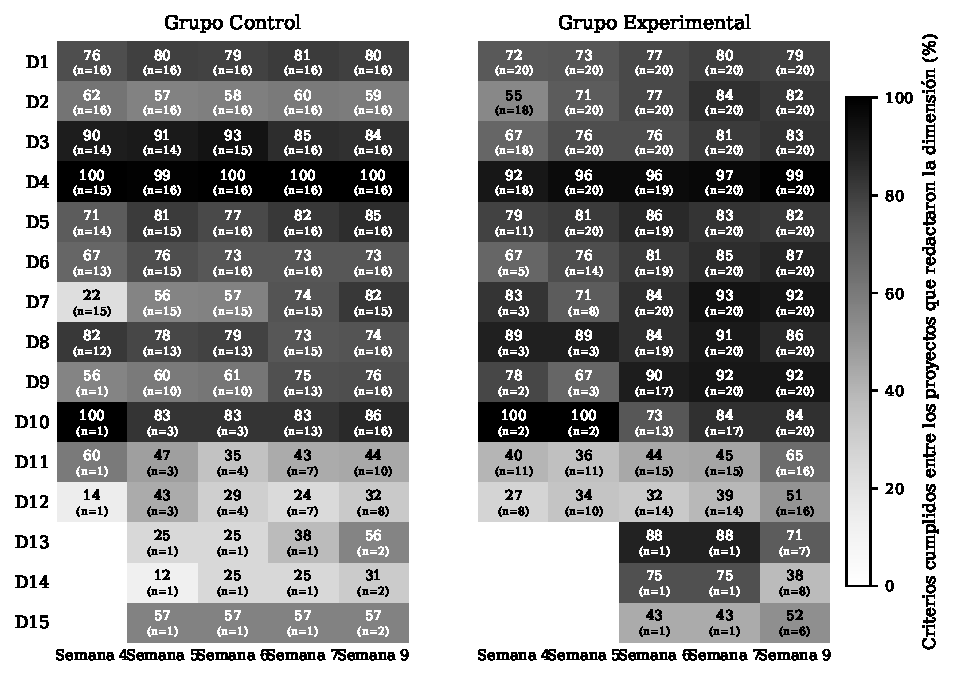
\includegraphics[width=0.92\textwidth]{../figuras/fig2_logro_por_dimension.pdf}
\caption{Logro por dimensión de la rúbrica de la semana 4 a la semana 9, por grupo. Porcentaje de criterios cumplidos entre los proyectos que redactaron cada dimensión en cada medición; entre paréntesis, el número de proyectos. D1 = título; D2 = descripción del problema; D3 = formulación del problema; D4 = objetivos; D5 = justificación; D6 = limitaciones; D7 = marco teórico; D8 = hipótesis; D9 = variables; D10 = matriz de consistencia; D11 = tipo de investigación; D12 = diseño; D13 = población y muestra; D14 = técnicas e instrumentos; D15 = procesamiento y análisis. La semana 8 no se midió.}
\label{fig:heatmap}
\end{figure*}

\subsection{Uso del sistema y su relación con la mejora}

Los 31 estudiantes del grupo experimental contaron con una cuenta y 18 de los 20 proyectos consultaron al sistema al menos una vez entre la semana 5 y la semana 9, con 215 consultas en total: 98 en la semana 5 (17 proyectos), 22 en la semana 6 (8 proyectos), 72 en la semana 7 (9 proyectos) y 23 en las semanas 8 y 9 (2 proyectos). Predominaron las consultas rápidas (106) y las mejoras rápidas (66), seguidas de las revisiones completas (28) y de sección (15). Se registraron 76 sesiones con consultas (2\,272 minutos) y 104 sesiones sin mensajes (697 minutos). El uso se concentró en pocos proyectos: cuatro de ellos reunieron 135 de las 215 consultas. En ninguno de los cuatro intervalos el número de consultas se relacionó de forma significativa con el cambio de la calidad sobre las dimensiones de la semana anterior ($\rho$ de Spearman entre $-.20$ y .24; $p$ unilateral entre .155 y .807), y el modelo de efectos mixtos del cambio por intervalo (80 intervalos) no mostró efecto del uso del intervalo ($b = -0.07$ puntos por consulta, $p = .759$) ni del anterior ($b = -0.10$, $p = .709$). La correlación entre el uso acumulado y el cambio total de la calidad entre la semana 4 y la semana 9 fue negativa y no significativa ($\rho = -.14$, $p = .725$, $n = 20$), al igual que con los días con consultas ($\rho = -.22$) y los minutos en sesiones con consultas ($\rho = -.25$). Los cuatro proyectos con mayor uso registraron cambios de $+3.2$, $+32.6$, $+8.7$ y 0.0 puntos, mientras que tres proyectos con menos de cinco consultas mejoraron más de 20 puntos (Fig.~\ref{fig:use}). En consecuencia, no se rechazó $H_0$ de la H3.

\begin{figure}[!t]
\centering
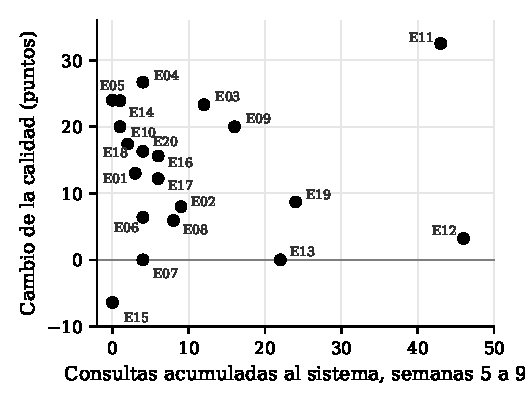
\includegraphics[width=\columnwidth]{../figuras/fig3_uso_vs_cambio.pdf}
\caption{Uso acumulado del sistema frente al cambio de la calidad entre la semana 4 y la semana 9 en el grupo experimental ($n = 20$). El cambio se calcula sobre las dimensiones que cada proyecto tenía redactadas en ambas mediciones. $\rho$ de Spearman $= -.14$; $p$ unilateral $= .725$.}
\label{fig:use}
\end{figure}

\subsection{Comparación de las trayectorias entre grupos}

La calidad en las dimensiones desarrolladas por ambos grupos fue de 78.5\,\% en el grupo de control y de 71.2\,\% en el experimental en la semana 4 (D1--D5); de 79.7\,\% y 79.5\,\% en la semana 5 (D1--D6); de 72.4\,\% y 83.6\,\% en la semana 6 (D1--D9); de 77.2\,\% y 88.2\,\% en la semana 7 (D1--D10); y de 75.6\,\% y 83.9\,\% en la semana 9 (D1--D12). Desde la semana 6 la calidad del grupo experimental superó a la del de control en cada medición (Fig.~\ref{fig:core}). En el modelo de efectos mixtos, la calidad del grupo experimental partió 2.22 puntos por debajo de la del grupo de control y su pendiente semanal fue 3.10 puntos mayor (Tabla~\ref{tab:mixed}), por lo que se rechazó $H_0$ de la H4. El cambio total sobre las dimensiones que cada proyecto ya tenía redactadas no difirió entre grupos (medianas de $+14.3$ y $+11.3$ puntos; $U = 161.0$, $p = .494$, $\delta = 0.01$): ambos grupos mejoraron de forma similar lo que ya tenían escrito, y la diferencia se originó en la calidad con la que el grupo experimental redactó las dimensiones incorporadas después de la medición inicial.

\begin{table}[!t]
\caption{Modelo lineal de efectos mixtos de la calidad en el núcleo común, de la semana 4 a la semana 9}
\label{tab:mixed}
\centering
\footnotesize
\begin{tabular}{L{3.0cm}rrcc}
\toprule
Término & $b$ & $EE$ & IC 95\,\% & $p$ \\
\midrule
Intercepto (grupo de control, semana 4) & 78.09 & 1.86 & $[74.44, 81.74]$ & $<.001$ \\
Grupo experimental & $-2.22$ & 2.50 & $[-7.12, 2.67]$ & .373 \\
Semana & $-0.64$ & 0.48 & $[-1.58, 0.31]$ & .187 \\
Grupo experimental $\times$ semana & 3.10 & 0.65 & $[1.83, 4.37]$ & $<.001$ \\
\bottomrule
\end{tabular}
\\[2pt]
\raggedright\scriptsize 180 observaciones de 36 proyectos; intercepto aleatorio por proyecto (varianza 26.42; varianza residual 55.09). $b$ en puntos porcentuales; la semana se cuenta desde la medición inicial, de modo que la semana 9 corresponde al valor 5. El valor $p$ de la interacción es unilateral ($H_1$: la pendiente del grupo experimental es mayor); los demás son bilaterales.
\end{table}

\begin{figure}[!t]
\centering
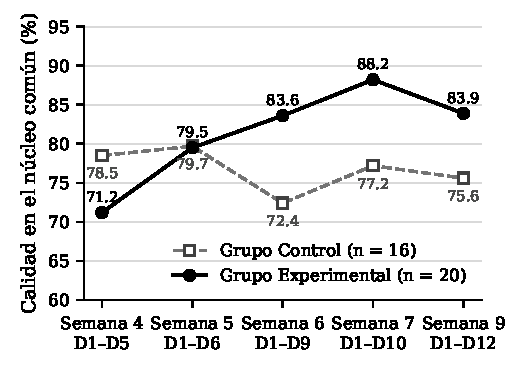
\includegraphics[width=\columnwidth]{../figuras/fig1_calidad_nucleo_comun.pdf}
\caption{Calidad media en el núcleo común de dimensiones en cada medición, por grupo. Bajo cada semana se indican las dimensiones del núcleo común de esa medición (D1 a D12 según la numeración de la rúbrica). La semana 8 no se midió.}
\label{fig:core}
\end{figure}

\subsection{Calidad argumentativa de la descripción del problema y de la justificación}

En la semana 4 se analizaron 33 descripciones del problema y 25 justificaciones completas, y en la semana 7, 36 de cada una. El modelo identificó una mediana de 5 afirmaciones del autor por descripción del problema; el 70.4\,\% de las afirmaciones tenía al menos un dato, el 6.5\,\% una garantía, el 2.2\,\% un respaldo, el 5.4\,\% un calificador y el 0.5\,\% una refutación, y en las justificaciones el 66.2\,\% tenía datos y el 5.5\,\% garantías. El 57.3\,\% de los vínculos unía unidades de párrafos distintos. Treinta y dos de las 33 descripciones del problema se ubicaron en el nivel 2 de Erduran \emph{et al.} \cite{erduran2004}, que corresponde a afirmaciones con fundamentos y sin refutación. En la semana 7 el perfil se mantuvo: el 81.2\,\% de las afirmaciones de la descripción del problema tenía datos y el 7.6\,\% garantías; en la justificación, el 74.5\,\% y el 4.5\,\%. La mediana del índice de elaboración de la descripción del problema pasó de 16.7\,\% a 20.0\,\% y la de la justificación, de 15.0\,\% a 18.0\,\%. El cambio del índice entre la primera y la última medición con la sección completa no fue mayor en el grupo experimental en la descripción del problema, pero sí en la justificación (Tabla~\ref{tab:argument}), por lo que la H5 se aceptó de forma parcial. Con el índice estructural, que solo toma siete valores, no se rechazó $H_0$ en ninguna sección ($p$ ajustados $= .645$ y .189). El índice de elaboración no se relacionó con la calidad de la dimensión correspondiente de la rúbrica (descripción del problema: $\rho = .04$ y .05; justificación: $\rho = .02$ y .22, en las semanas 4 y 7), lo que indica que recoge una información distinta de la que verifica la rúbrica.

\begin{table*}[!t]
\caption{Índice de elaboración argumentativa por sección y grupo, de la semana 4 a la semana 7}
\label{tab:argument}
\centering
\footnotesize
\begin{tabular}{L{2.6cm}L{2.8cm}cccccc}
\toprule
Sección & Grupo & $Mdn$ S4 & $Mdn$ S7 & Cambio ($Mdn$) & $U$ & $p$ (Holm) & $\delta$ \\
\midrule
\multirow{2}{=}{Descripción del problema} & Control ($n = 16$) & 18.4 & 20.0 & $+2.5$ & \multirow{2}{*}{156.5} & \multirow{2}{*}{.551 (.551)} & \multirow{2}{*}{$-.02$} \\
 & Experimental ($n = 20$) & 16.7 & 20.0 & $+3.1$ & & & \\
\addlinespace
\multirow{2}{=}{Justificación} & Control ($n = 16$) & 15.2 & 15.3 & $-1.4$ & \multirow{2}{*}{230.0} & \multirow{2}{*}{.013 (.027)} & \multirow{2}{*}{$+.44$} \\
 & Experimental ($n = 20$) & 10.0 & 20.0 & $+3.1$ & & & \\
\bottomrule
\end{tabular}
\\[2pt]
\parbox{0.92\textwidth}{\raggedright\scriptsize Índice de elaboración en porcentaje: media, sobre las afirmaciones de la sección, de la proporción de los cinco componentes de apoyo que tiene cada una. El cambio se calcula entre la primera y la última medición en que la sección está completa. Prueba $U$ de Mann-Whitney unilateral ($H_1$: el cambio es mayor en el grupo experimental), con el valor $p$ ajustado por el método de Holm para las dos secciones; $\delta$ = delta de Cliff.}
\end{table*}

\subsection{Efecto del sistema sobre la calidad metodológica}

La calidad en el núcleo común de cada medición cambió, entre la semana 4 (D1--D5) y la semana 9 (D1--D12), en promedio $+12.6$ puntos ($DE = 11.0$) en el grupo experimental y $-2.9$ puntos ($DE = 12.6$) en el grupo de control. Los cambios de ambos grupos fueron normales (Shapiro-Wilk, $p = .810$ y .795) y con varianzas homogéneas (Levene, $p = .568$). La diferencia equivale a una $d$ de Cohen de 1.32 (IC 95\,\% $[0.60, 2.05]$; desviación estándar combinada de 11.7 puntos), un efecto grande cuyo límite inferior corresponde a un efecto mediano, y la prueba $t$ de Student unilateral arrojó $t(34) = 3.94$, $p < .001$; se rechazó $H_0$ de la hipótesis general. Por dimensión, el efecto a favor del grupo experimental fue al menos mediano en ocho de las doce dimensiones del núcleo final (Tabla~\ref{tab:effect}); fue despreciable en el título y la matriz de consistencia, y favorable al grupo de control en la justificación. Sobre lo que cada proyecto ya tenía escrito en la semana 4, el efecto fue despreciable ($d = -0.06$; IC 95\,\% $[-0.72, 0.59]$).

\begin{table*}[!t]
\caption{Tamaño del efecto del sistema por dimensión de la rúbrica}
\label{tab:effect}
\centering
\footnotesize
\begin{tabular}{L{3.4cm}L{2.4cm}ccrrL{2.6cm}L{1.8cm}}
\toprule
Dimensión & Medida & $n_{\mathrm{GC}}$ & $n_{\mathrm{GE}}$ & GC $M$ (\%) & GE $M$ (\%) & $d$ [IC 95\,\%] & Magnitud \\
\midrule
D1 Título & Cambio S4--S9 & 16 & 20 & 3.8 & 7.0 & $0.14$ $[-0.52, 0.80]$ & Despreciable \\
D2 Descripción del problema & Cambio S4--S9 & 16 & 18 & $-3.1$ & 28.5 & $1.03$ $[0.31, 1.75]$ & Grande \\
D3 Formulación del problema & Cambio S4--S9 & 14 & 18 & $-5.7$ & 15.6 & $0.72$ $[0.00, 1.44]$ & Mediano \\
D4 Objetivos & Cambio S4--S9 & 15 & 18 & 0.0 & 6.3 & $0.97$ $[0.25, 1.70]$ & Grande \\
D5 Justificación & Cambio S4--S9 & 14 & 11 & 15.5 & 7.6 & $-0.32$ $[-1.12, 0.47]$ & Pequeño \\
D6 Limitaciones & Nivel en S9 & 16 & 20 & 72.9 & 86.7 & $0.66$ $[-0.01, 1.34]$ & Mediano \\
D7 Marco teórico & Nivel en S9 & 15 & 20 & 81.7 & 92.5 & $0.86$ $[0.16, 1.55]$ & Grande \\
D8 Hipótesis & Nivel en S9 & 16 & 20 & 74.0 & 85.8 & $0.40$ $[-0.26, 1.06]$ & Pequeño \\
D9 Variables & Nivel en S9 & 16 & 20 & 76.4 & 92.2 & $0.92$ $[0.23, 1.61]$ & Grande \\
D10 Matriz de consistencia & Nivel en S9 & 16 & 20 & 85.9 & 83.8 & $-0.10$ $[-0.76, 0.56]$ & Despreciable \\
D11 Tipo de investigación & Nivel en S9 & 10 & 16 & 44.0 & 65.0 & $0.81$ $[-0.01, 1.63]$ & Grande \\
D12 Diseño del estudio & Nivel en S9 & 8 & 16 & 32.1 & 50.9 & $0.84$ $[-0.04, 1.72]$ & Grande \\
\bottomrule
\end{tabular}
\\[2pt]
\parbox{0.92\textwidth}{\raggedright\scriptsize GC = grupo de control; GE = grupo experimental. En las dimensiones de la medición inicial (D1 a D5) se compara el cambio del logro entre la semana 4 y la semana 9, en puntos porcentuales, entre los proyectos que las tenían redactadas en ambas mediciones; en las incorporadas después, el logro en la semana 9 entre los proyectos que las redactaron. $d$ = GE $-$ GC; magnitud según Cohen \cite{cohen1988}: despreciable por debajo de 0.20, pequeño desde 0.20, mediano desde 0.50, grande desde 0.80.}
\end{table*}

\section{Discusión}

El estudio encontró que los proyectos del grupo que dispuso del sistema multiagente evolucionaron de forma significativamente más favorable que los del grupo con asesoría tradicional, con un efecto grande sobre el cambio de la calidad en el núcleo común de dimensiones ($d = 1.32$). Dos precisiones delimitan ese hallazgo. La primera es que la mejora no fue exclusiva del grupo experimental: la calidad de lo ya redactado aumentó en ambos grupos en magnitud similar, lo que indica que el avance del curso, la asesoría y la retroalimentación en clase actúan sobre ambos, y que el efecto del sistema se concentró en la descripción del problema y en la calidad con la que se redactaron las dimensiones incorporadas durante la intervención (limitaciones, marco teórico, variables, tipo y diseño de investigación). El sistema se asocia más con la calidad con la que se escribe lo nuevo que con la corrección de lo ya escrito. La segunda es que el efecto debe interpretarse frente a la práctica habitual del curso y no frente a la ausencia de herramientas, porque el estudio no restringió ni registró el uso de otras herramientas de inteligencia artificial en ninguno de los grupos.

El resultado se alinea con J.\ Du \emph{et al.} \cite{duj2025}, que reportaron una mayor mejora relativa del aprendizaje con un sistema de debate entre agentes, aunque en el aprendizaje de contenidos y no en la calidad de un documento de investigación, y contrasta con Apolín Montes \emph{et al.} \cite{apolin2024}, quienes, con un grupo de control no equivalente y dos mediciones, no encontraron diferencias en la producción de textos académicos con un modelo conversacional de propósito general. La divergencia es coherente con el diagnóstico de los asesores y con los antecedentes cualitativos: las funciones que se esperan de una herramienta de apoyo, la revisión de coherencia entre problema, objetivos, variables e hipótesis y las sugerencias basadas en evidencia, exceden la capacidad de un agente conversacional genérico, que tiende a operar como dispensador de recursos \cite{ortega2021} o a fallar ante consultas de contenido complejo \cite{arredondo2020}. A diferencia del diseño preexperimental de Hinojosa Mamani \emph{et al.} \cite{hinojosa2024}, que atribuyó la mejora a la intervención sin grupo de comparación, el diseño con grupo de control y cinco mediciones permitió separar la mejora común a ambos grupos de la asociada al sistema y observar que las trayectorias se separan desde la semana 6 y que la ventaja se mantenía cinco semanas después de la medición inicial, lo que responde a la recomendación de Deng \emph{et al.} \cite{deng2025} de evaluar estos efectos a lo largo del tiempo. En el plano de la medición, el nivel metodológico intermedio observado al inicio (entre el 65\,\% y el 67\,\% de los criterios aplicables cumplidos) coincide con la calidad regular que Estrada Araoz \emph{et al.} \cite{estrada2022} hallaron en tesis ya aprobadas, y la concentración de incumplimientos en la descripción del problema confirma con medición directa lo que los asesores atribuyeron a que el estudiante parte de la solución tecnológica.

La ausencia de relación entre el nivel de uso y la mejora dentro del grupo experimental obliga a interpretar el efecto como el de disponer del sistema y no como una relación de dosis y respuesta. El uso fue reducido y se concentró en pocos proyectos, patrón compatible con la adopción limitada documentada por Arredondo Castillo \cite{arredondo2020} y con el registro de uso sin vinculación con la calidad de Artiles Rodríguez \emph{et al.} \cite{artiles2021}; Sánchez-Vera \cite{sanchezvera2025} encontró, además, que un uso moderado de un chatbot especializado se asoció con mejores resultados y que el uso excesivo no añadió mejoras, lo que sugiere que la relación entre dosis y resultado no es lineal. Solo uno de los cuatro proyectos de mayor uso figura entre los cinco que más mejoraron, de modo que el número de consultas no recoge por sí solo la forma en que cada estudiante incorporó las respuestas del sistema a su proyecto. En el plano argumentativo, las afirmaciones de ambos grupos se sostienen sobre todo con datos y rara vez con garantías, respaldos o refutaciones, perfil que se mantuvo de la semana 4 a la semana 7 y que precisa el planteamiento superficial del problema descrito por los asesores. El índice de elaboración de la justificación aumentó más en el grupo experimental, pero no el de la descripción del problema, y su independencia respecto de la rúbrica indica que una sección puede cumplir los criterios exigidos sin sostener sus afirmaciones, información que la rúbrica no recoge y que, siguiendo a Wambsganss \emph{et al.} \cite{wambsganss2020}, podría orientar la mentoría hacia la garantía y el respaldo.

Respecto del estado del arte, el estudio aporta la primera evidencia controlada y longitudinal, en un curso real de ingeniería en el Perú, sobre un sistema multiagente especializado en mentoría metodológica, con un instrumento validado por juicio de expertos, un evaluador automatizado con consistencia reportada en cada medición y una evaluación computacional de la argumentación de las secciones del proyecto. No lo supera en términos de generalización: el tamaño de la muestra, la asignación por secciones intactas y la homogeneidad inicial parcial limitan la validez externa e interna de las comparaciones entre grupos. La Tabla~\ref{tab:gaps} resume el grado en que los resultados cubren las brechas identificadas; ninguna se declara cerrada, dado que las dimensiones metodológicas, las de mayor exigencia, aún no se desarrollan en la mayoría de los proyectos y la relación entre el uso y la mejora no se ha establecido.

\begin{table}[!t]
\caption{Brechas de investigación atendidas y grado de cobertura}
\label{tab:gaps}
\centering
\footnotesize
\begin{tabular}{cL{2.7cm}L{2.9cm}L{1.25cm}}
\toprule
OE & Brecha & Aporte del estudio & Cobertura \\
\midrule
1 & Escasa evidencia desde la perspectiva del asesor de ingeniería y sin diagnóstico por sección en la etapa de proyecto & Entrevistas a seis asesores con saturación en seis categorías; deficiencias por sección, limitaciones operativas y funcionalidades esperadas & Sustancial (70--80\,\%) \\
2 & Calidad medida en un único momento, sin evolución por componente & Mismo instrumento aplicado a los mismos proyectos en cinco mediciones; logro por dimensión en cada una & Parcial (50--55\,\%) \\
3 & Registros de uso sin vinculación con la calidad de productos de investigación & Dosis de uso por proyecto y semana vinculada con el cambio de la calidad; sin relación positiva & Parcial (45--50\,\%) \\
4 & Predominio de diseños pretest-postest; escasa evidencia controlada sobre sistemas multiagente especializados & Cinco mediciones comparadas con un modelo de efectos mixtos; efecto grande con grupo de control & Parcial (50\,\%) \\
5 & Evaluación computacional de la argumentación desarrollada sobre ensayos y en un único momento & Índice argumentativo con vínculos entre párrafos y verificación automática, medido en cuatro mediciones y relacionado con la rúbrica & Sustancial a parcial (50--65\,\%) \\
\bottomrule
\end{tabular}
\\[2pt]
\raggedright\scriptsize OE = objetivo específico. Escala de cobertura: 40\,\% a 50\,\%, parcial; 65\,\% a 80\,\%, sustancial con componentes pendientes; 85\,\% a 100\,\%, cerrada. Cobertura global de las diez brechas: 56.5\,\%.
\end{table}

\subsection{Limitaciones}

El diseño trabajó con secciones intactas sin asignación aleatoria de los proyectos, y la homogeneidad inicial fue parcial: el grupo de control partió con mayor trazabilidad y con una calidad del núcleo moderadamente mayor ($g = -0.65$), de modo que parte de la convergencia puede deberse a la regresión hacia la media; por ello las comparaciones se apoyaron en el cambio de cada proyecto respecto de su propia medición inicial y en un modelo que estima por separado el nivel y la pendiente. Factores propios de cada sección, como su composición, el día y el ritmo de la clase, la asesoría externa o el uso de otras herramientas de inteligencia artificial, no quedaron controlados; en la semana 6, además, la asesoría a ambos grupos fue mínima. Los resultados corresponden a una sola facultad y a cinco mediciones de una serie que continúa hasta la primera versión completa de los proyectos, y las dimensiones de la metodología aún no cuentan con suficiente desarrollo para analizar su evolución. El sistema evaluador fue el único aplicador de la rúbrica: su validez se sustenta en la validación de contenido del instrumento y en el carácter dicotómico de los ítems, pero sus calificaciones no se contrastaron con calificadores humanos. Los tres jueces pertenecen a la misma familia de modelos y al menos uno de ellos forma parte de los modelos que emplea el sistema de mentoría, por lo que el panel no neutraliza el sesgo de autopreferencia \cite{panickssery2024}; el riesgo se mitigó con temperatura 0, semilla fija, criterios dicotómicos y voto de mayoría, sin eliminarlo. La variabilidad entre jueces fue moderada (kappa de Fleiss entre .46 y .66). El índice argumentativo registra la presencia de los componentes y no su solidez, su estabilidad test-retest fue moderada (CCI $= .77$) y su contraste con una anotación humana está pendiente; la aceptación parcial de la H5 depende del índice continuo y debe interpretarse con cautela.

\subsection{Trabajo futuro}

Se sugiere replicar el diseño en otras escuelas y universidades con muestras mayores y asignación aleatoria por conglomerados; completar la serie longitudinal hasta la versión final de los proyectos para analizar las dimensiones metodológicas; contrastar las calificaciones del panel con calificadores humanos sobre una submuestra, con intervalos de confianza por remuestreo \emph{bootstrap}; conformar los paneles de jueces con modelos de familias distintas entre sí y distintas del modelo generador; registrar el uso de otras herramientas de inteligencia artificial en ambos grupos; analizar los mismos datos con indicadores de uso que recojan la incorporación efectiva de las respuestas del sistema al documento; y validar el índice argumentativo con anotación humana de las mismas secciones.

\section{Conclusiones}

\begin{enumerate}
\item El diagnóstico cualitativo identificó la formulación del problema y el marco metodológico como las secciones de mayor incidencia de errores, y la naturaleza puntual de la asesoría como la principal limitación estructural de la mentoría tradicional; las funcionalidades que los asesores esperan de una herramienta de apoyo exceden la capacidad de un agente conversacional genérico y respaldan la elección de una arquitectura multiagente especializada anclada en una rúbrica.
\item La calidad metodológica de los proyectos aumentó de forma significativa entre la semana 4 y la semana 9 en 32 de 36 proyectos (mediana $+13.0$ puntos; $p < .001$), en ambos grupos, con deficiencias iniciales concentradas en la descripción del problema; la medición se sustentó en una rúbrica con validez de contenido (V de Aiken entre .81 y 1.00).
\item El nivel de uso del sistema, reducido y concentrado en pocos proyectos (215 consultas), no se relacionó con la mejora de la calidad en el grupo experimental ($\rho = -.14$; $p = .725$), por lo que el efecto no muestra una relación de dosis y respuesta.
\item La calidad en las dimensiones desarrolladas por ambos grupos evolucionó de forma significativamente más favorable en el grupo experimental, con una pendiente semanal 3.10 puntos mayor ($p < .001$); la diferencia se originó en las dimensiones incorporadas después de la medición inicial.
\item Las afirmaciones de la descripción del problema y de la justificación se sostienen con datos y rara vez con garantías, respaldos o refutaciones; el índice de elaboración de la justificación aumentó más en el grupo experimental ($p$ ajustado $= .027$), no así el de la descripción del problema, por lo que la H5 se aceptó de forma parcial.
\item El sistema multiagente tuvo un efecto positivo, estadísticamente significativo y grande sobre la calidad metodológica de los proyectos de tesis ($d = 1.32$; IC 95\,\% $[0.60, 2.05]$; $p < .001$), concentrado en la descripción del problema y en las dimensiones redactadas durante la intervención, que se interpreta como el efecto de disponer del sistema frente a la práctica habitual del curso. Como implicancia práctica, los sistemas de mentoría automatizada deberían priorizar el refuerzo de la descripción y formulación del problema, y la facultad debería considerar mecanismos de estandarización de criterios entre asesores y jurados, cuya divergencia alcanzó saturación plena en el diagnóstico.
\end{enumerate}

\section*{Agradecimientos}

Los autores agradecen a los docentes y asesores de la Facultad de Ingeniería de la UPAO que participaron en las entrevistas y en la validación del instrumento, al docente del curso Proyecto de Investigación por facilitar la aplicación del estudio en sus secciones, y a los estudiantes que autorizaron la evaluación de sus proyectos. Los modelos de lenguaje descritos en la sección~II forman parte del objeto de estudio; no se empleó inteligencia artificial generativa para tomar decisiones de investigación.

\section*{Disponibilidad de datos y código}

El código fuente del sistema de mentoría está disponible en \url{https://github.com/Mclever2/MentorIA-Tesis}. La rúbrica de 100 ítems con sus coeficientes V de Aiken, la guía de entrevista, los resultados por proyecto en cada medición, los estadísticos de consistencia del panel y los registros de uso agregados por proyecto y semana se proporcionan como material suplementario.

\bibliographystyle{IEEEtran}
\bibliography{references}

\begin{IEEEbiographynophoto}{Clever Josu\'e Aguilar Idrogo}
es candidato al título profesional de Ingeniero de Computación y Sistemas por la Universidad Privada Antenor Orrego, Trujillo, Perú. Sus intereses de investigación incluyen los sistemas multiagente basados en modelos de lenguaje, la generación aumentada por recuperación y la inteligencia artificial aplicada a la educación superior.
\end{IEEEbiographynophoto}

\begin{IEEEbiographynophoto}{Alessia Vidamilagros Aguilar Alayo}
es candidata al título profesional de Ingeniera de Computación y Sistemas por la Universidad Privada Antenor Orrego, Trujillo, Perú. Sus intereses de investigación incluyen la tecnología educativa, la evaluación automatizada de la escritura académica y los sistemas inteligentes.
\end{IEEEbiographynophoto}

\begin{IEEEbiographynophoto}{Walter Manuel Cueva Ch\'avez}
es docente de la Facultad de Ingeniería de la Universidad Privada Antenor Orrego, Trujillo, Perú, donde asesora proyectos de tesis de pregrado del Programa de Ingeniería de Computación y Sistemas. Sus intereses de investigación incluyen la metodología de la investigación, los sistemas inteligentes y la ingeniería de software.
\end{IEEEbiographynophoto}

\end{document}
